\documentclass[12pt, a4paper, lithuanian]{article}
\usepackage[utf8x]{inputenc}
\def\LTfontencoding{L7x}
\PrerenderUnicode{ąčęėįšųūž}
\usepackage[\LTfontencoding]{fontenc}
\usepackage[lithuanian]{babel}
\usepackage{VUMIFPSkursinis}
\usepackage{cite}
\usepackage{amsmath}
\usepackage{bm}
\usepackage{amsfonts}
\usepackage{float}
\usepackage{graphicx}
\usepackage{color}
\usepackage{listings}
\usepackage{wrapfig}
\usepackage{algpseudocode}
\usepackage{algorithm}
\usepackage{algorithmicx}
\usepackage{caption}
\usepackage{subfig}


% Titulinio aprašas
\vumifdept{Programų sistemų katedra}
\vumifpaper{Kursinis darbas}
\title{Programų sistemų kūrimo metodų tyrimas}
% \title{Esama situacija su dviem sluoksniais}
% \title{Ištirti selektyvios membranos įtaką amperometrinio bijojutiklio jautriui}
\def\titleineng{Investigation of software engineering methods}
\def\statusas{% Kai kurioms katedroms reikia nurodyti  
    2 kurso 1 grupės studentas \\
}
\author{
   Vardaitis Pavardaitis 
}

\supervisor{prof. habil. dr. Vardenis Pavardenis}
\date{Vilnius – \the\year}

\begin{document}
\sloppy
\maketitle

\tableofcontents


\vumifsectionnonum{Terminai}
\begin{enumerate}
\item ANT - klasikinis atgalinio perdavimo neuroninis tinklas (angl.
back-propagation neural network)
\item DNT - dirbtinis neuroninis tinklas (angl. artificial neural network)
\item DSP - daugiasluoksnis perceptronas (angl. multilayer perceptron)
\item ...
\end{enumerate}


\vumifsectionnonum{Įvadas}
Įvadas.


\section{Skyriaus pavadinimas}
Skyriaus tekstas. \cite{Banerjee1997}


\bibliography{bibliografija}


\appendix
\section{Papildomų eksperimentų rezultatų lentelės}
\begin{figure}[H]
    \centering
    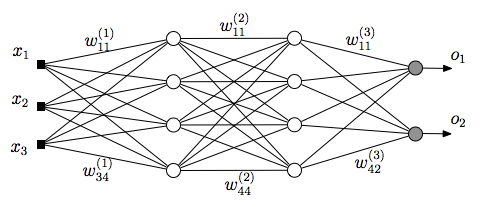
\includegraphics[scale=0.5]{img/MLP}
    \caption{Paveikslėlio pavyzdys}
    \label{img:mlp}
\end{figure}

\end{document}
